\documentclass[12pt]{article}
\usepackage[english]{babel}
\usepackage[pdftex]{graphicx}
\usepackage[latin1]{inputenc}
\usepackage{verbatim}
\usepackage{listings}
\usepackage{amsfonts}
\usepackage{color}
\usepackage{epsfig}
\usepackage{fancyvrb}
\usepackage{listings}
\date{}

\lstset{
  %backgroundcolor=\color{gray},
  frameround=fttt,
  stringstyle=\ttfamily,
  language=python,
  basicstyle=\small
}

\newcommand{\bigtilde}{$\sim$}
%% \def\framework{\textsc{Report}}

%\advance\textwidth by -1truecm
%\advance\oddsidemargin by 1truecm
%\advance\baselineskip by \baselineskip

\begin{document}

\begin{titlepage}
%%   \pagecolor{unih}
  \begin{center}
%%    \textbf{\uppercase{University of HertfordShire}}\\
%%     \hbox to \textwidth{\hrulefill}    
    %\fbox{
    \uppercase{ \textsf{
        \LARGE{REAR} \\ 
        \vspace{0.5truecm}
        \large{an exocentric vision framework for mobile robot teleoperations}
    }}
    %}              
    \hbox to \textwidth{\hrulefill}
    \vfill
    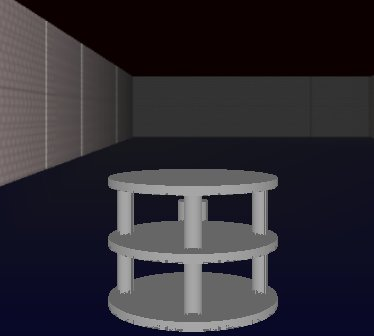
\includegraphics[width=250pt]{img/rear_snapshot.jpg}
    \vfill
    
    \begin{flushright}
      \textsf{Students:} \\
      \textsf{\textbf{Daniele Ferro}} \\                      
      \textsf{\textbf{Loris Fichera}}
      \vspace{0.5 truecm}
                
      \textsf{Supervisor:} \\
      \textsf{\textbf{Prof. Salvatore Livatino }}\\
      \textsf{\textbf{Prof. Giovanni Muscato }}\\
    \end{flushright}
    
    \vspace{0.5 truecm}
    %%    \begin{figure}
    \hfill 
\includegraphics[width=300pt]{img/uni_logo.jpg}  %logo
%%    \end{figure}
    
  \end{center}
  
\end{titlepage}

\setlength{\baselineskip}{1.3\baselineskip} %per 30 righe in ogni pag.

\tableofcontents

\newpage
  % Frontpage
\section{State of the art}
\label{stateart}
%

%
Display used for common Head Mounted Display (HMD) are 
various, we try to explain the chief differences. In the
following we will examine five types: LCD, AMLCD, LCOS, 
FLCOS, OLED.
%

%
\subsection{LCD}
The LCD technology is based on the light modulating properties 
of liquid crystals (LCs). Since LCs are not able to emit light 
directly, actual LCD panels and displays need a light source.
%
That is why such devices are often classified as "passive" 
displays. 
%
LCD displays are usually for a general purpose use, but they 
can also be tuned for a specific usage - e.g. the displaying 
of highly detailed still images or of highly dynamic, 
fast-changing video content.
%
Because of their versatility, they are used in a wide range 
of applications including computer monitors, TVs, aircraft 
cockpits. They're also common in electronic consumer devices 
such as video player, gaming devices, etc.
%
Compared to other display-making technologies - such as CRT - 
LCD allows to make wider and flatter displays while reducing 
electrical power consumption and, thus, making LCD displays 
also well-suitable for mobile devices.
%

%
\subsection{AMLCD}
Active Matrix LCDs (AMLCD) use a matrix of thin-film transistors 
(TFTs) to achieve better performance compared to normal LCD screens. 
They still have polarizing sheets and cells of liquid crystal 
(same as LCD), but the TFTs allow to store the electrical state 
of each pixel on the display while all the other pixels are 
being updated.
%
The advantages of a TFT-LCD monitor are many. It provides a 
larger viewing-angle and a much brighter display than a passive 
matrix monitor with the same size. Some designs have replaced 
transistors with other components such as diodes.
%
With an active matrix only the desired pixel receives a charge, 
acting as a capacitor and holding the charge until the next refresh 
cycle (transistors have the ability to hold a charge for a limited 
period of time). On the contrary, a passive matrix display delivers 
current to the liquid crystals in a specific area with a simple 
conductive grid. AMLCD can be more accurate because, thanks to 
the switching action of transistors, only a the specific pixels 
receive a charge, improving image quality with respect to a 
passive matrix display.
%
AMLCDs are most popular type of display on the market today.

\subsection{LCOS}
Liquid crystal on silicon (LCOS) is a {\it micro-projection} or 
{\it micro-display} technology typically applied in projection 
televisions. It is a reflective technology and uses liquid crystals.
%
LCoS displays are well-suited for high resolution and high contrast 
images. 
%
There are two broad categories of LCoS displays: three-panel and 
single-panel. In three-panel designs, there is one display chip 
per color, and the images are combined optically. Single-panel 
designs, instead, makes use of only one display chip  that shows 
the red, green, and blue components in succession with the 
observer's eyes relied upon to combine the color stream. 
%
If the frequency of the color fields is lower than about 540 Hz, 
an effect called "color breakup" is seen, where false colors 
are briefly perceived when either the image or the observer's 
eye is in motion.
%

%
\subsection{FLCOS}
FLCOS devices are made using ferroelectric liquid crystals 
(so the technology is named FLCoS), which are inherently faster 
than other types of liquid crystals.
%

%
\subsection{OLED}
The Organic Light Emitting Diode (OLED) takes advantage of an 
electroluminescent layer, made of organic compounds, used 
like a LED. This layer is wrapped between two electrodes and 
at least one of the electrodes is transparent.
%
OLEDs are a young display technology, not yet able to emit as 
much light per unit area as an inorganic solid-state based LED. 
For this reason OLED are not used as point-light sources.
%
This devices can be used for multiple applications, from 
television and computer screens to small and portable system 
screens such as mobile phones, PDAs and head-mounted displays 
(where high-resolution is needed).
%
Since OLED displays do not require a backlight, they can 
perform deep black levels and be thinner and lighter than 
LCD panels. Besides, OLED displays can achieve higher contrast 
ratios. Even the power drain is lower, compared to LCD screen.
%

%
\subsection{A comparison towards displays}
By using AMLCD display for Head Mounted Display (HMD) the entire 
device is more compact, because AMLCDs only need a flat backlit 
panel rather than a complex (and thicker) illumination unit. 
This is the reason why FLCOS and LCOS displays are commonly not used. 
%
On the other hand, AMLCD display has relatively low contrast ratio 
and provides the lowest luminance range and largest pixel dimensions 
among all of the previously seen technologies.
As well as AMLCD, OLED offer a compact system design due to its 
self-emission nature. In addition, OLEDs provide a good range of 
luminance, even tough the resolution and contrast ratio of 
existing OLEDs are relatively low compared with FLCOS and LCOS microdisplays.
%
Besides, OLEDs life span would be shortened if the display 
luminance is high (e.g. more than 100 cd/m2).
%
According to \cite{Zhang:08}, for HMD designs a display panel around 2.50 cm is 
preferable as it would offer a good balance of compactness and the 
focal length range of the optics. In fact, when dealing with small 
display panels, shorter focal length and larger magnification are 
required in order to achieve a reasonable field-of-view (FOV). 
%
LCOS microdisplays offer the highest resolution and contrast compared 
with other types of displays and they are commonly used as image 
sources in digital projectors. 
%

%
\begin{figure}[!h]
  \begin{center}
    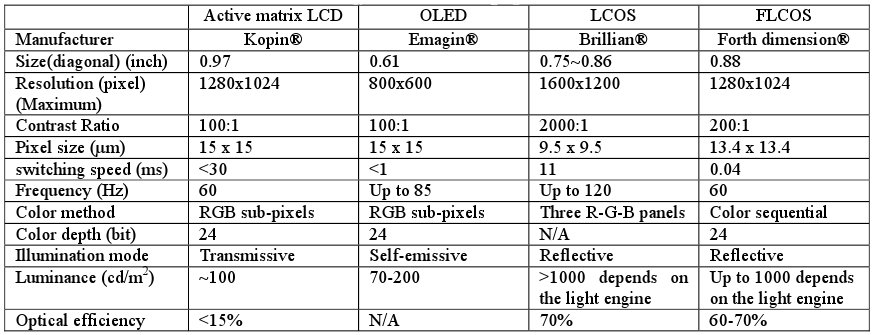
\includegraphics[width=400pt]{img/hmd_comparison_table}  %logo
  \end{center}
\end{figure}
%

%
The liquid crystal used in LCOS microdisplays, however, has low 
switching speed, which makes it impossible to use color sequential 
method, to achieve a full color mode. FLCOS offers high pixel 
resolution, luminance output, image contrast, and optical efficiency. 
Also, the fast response speed of ferroelectric liquid crystal makes 
it possible to achieve full-color display using a single-panel color 
sequential scheme. On the other hand, it requires a carefully designed 
illumination unit to achieve high contrast and high luminance, which 
makes the overall display system less compact than a system using 
AMLCD or OLED microdisplays.

\setcounter{figure}{0}
\setcounter{table}{0}
\setcounter{lstlisting}{0}

\section{The Exocentric vision issue}
\label{sec:exo}

\section{Why exocentric vision ?}
\label{exo:why_exocentric}

Teleoperated mobile robots prove to be extremely useful 
when there is the need for performing operations in places that 
are inaccessible or dangerous for human beings - e.g. 
search-and-rescue missions within unknown regions or into 
collapsed buildings, caves, etc.
\\
The supervisors' research group has been widely involved 
during the last years in such a field: \cite{livatino2010}.
As testing platform, they have been using \morduc{},
a differential-driven mobile robot - see chapter \ref{intro:3morduc} -
equipped with a pair of \textit{Videre Design} \cite{videredesign} 
stereo cameras and a laser scanner.
\\
They have been focused 
mainly on the making of a reliable hardware and software 
infrastructure which could make a remote operator able to drive 
the \morduc{} in comfort.
\\
Indeed, our work focuses on \textit{robot-operator interaction} and, 
hence, on how to improve such interaction. 
\\
Analyzing previous work and data produced by the supervisors' 
research group, it emerges that the stereo cameras mounted on 
top of \morduc{} were used to provide the remote operators a 
\textit{first-person} point of view. In literature, such a 
system is also called an \textit{egocentric} vision system.
\\
According to \cite{sugimoto}, \textit{by observing the camera image 
without an efficient human interface system, the operator 
tends to misinterpret the robot's position and direction}. This is 
due to the fact that \textit{it's difficult for an
operator not accustomed to the vehicle to estimate the
vehicle's position and direction and the distances to a
target strictly based on camera images from the first person 
viewpoint}.
\\
In order to improve the interaction between the robot and the operator 
an exocentric camera would be effective since it would provide a 
view of the robot in the operating environment and, thus, 
a better understanding of where the robot is located into the
environment and its actual direction.
\\
Unfortunately the use of an exocentric camera is not straightforward: 
for example, it could be mounted on a rear-mounted protuberance of the 
robot, but such a protuberance would terribly limit the robot activity and 
its moving abilities.
\\
To avoid such complications, \cite{sugimoto} proposes 
\textit{Time Follower's}, an approach to provide a \textit{virtual exocentric 
view} of a mobile robot.


\subsection{Time Follower's: an overview}
\label{exo:why_exocentric::time_follower}

Time Follower's aims at providing an exocentric view of a mobile 
robot using an egocentric-mounted camera. The approach is simple: it is 
based on the use of previously recorded first-person images to provide 
comprehensible third-person imagery. A 3D representation of the robot 
is overlapped to such images in order to get the work done. A graphical
representation of the system is depicted in figure \ref{fig:exocentric}, 
while figure \ref{fig:virtualexocentric} shows an example of what appears 
to the end user.
\begin{figure}[!h]
  \begin{center}
    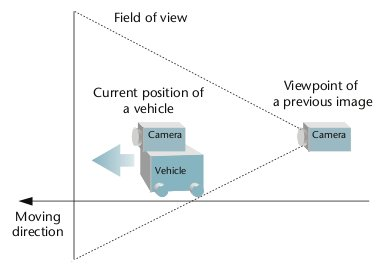
\includegraphics[width=200pt]{img/exocentric_vision.jpg}
    \caption{The \morduc{} robotic platform}
    \label{fig:exocentric}
  \end{center}
\end{figure}

\begin{figure}[!h]
  \begin{center}
    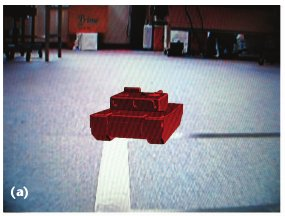
\includegraphics[width=200pt]{img/virtual_exocentric.jpg}  %robot pic
    \caption{A virtual exocentric vision example}
    \label{fig:virtualexocentric}
  \end{center}
\end{figure}

Key issues of such a system are:

\begin{itemize}
\item how to choose the \textit{best} image
\item how to determine the \textit{right} place to draw the robot
\end{itemize}

As for the first issue, the \textit{best} image is the one that allows 
the generation of the \textit{most comprehensible} external robot view.
\cite{sugimoto} provides a set of three effective metrics to 
determine which, of a set of previously recorded images, is the 
one to be chosen.
\\
Once the image is chosen, where to overlap the 3D robot representation 
is quite complex. It is not only a matter of \textit{where} draw the robot
on the image, but also of \textit{how} to set up lighting, robot dimensions,
perspective to make the end user not aware of the fact that what he is
seeing is not the actual environment.
\\
The issues introduced above will be deeply analyzed in the following 
of this document.

\newpage

\section{Time Follower's: an overview}
\label{exo:time_follower}

Time Follower's aims at providing an exocentric view of a mobile 
robot using an egocentric-mounted camera. The approach is simple: it is 
based on the use of previously recorded first-person images to provide 
comprehensible third-person imagery. A 3D representation of the robot 
is overlapped to such images in order to get the work done. A graphical
representation of the system is depicted in figure \ref{fig:exocentric}, 
while figure \ref{fig:virtualexocentric} shows an example of what appears 
to the end user.

\begin{figure}[!h]
  \begin{center}
    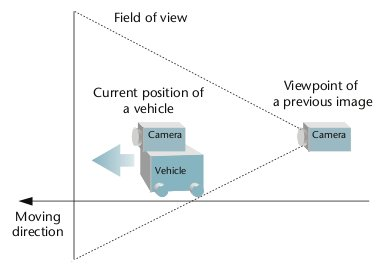
\includegraphics[width=200pt]{img/exocentric_vision.jpg}
    \caption{The Morduc robotic platform}
    \label{fig:exocentric}
  \end{center}
\end{figure}

\begin{figure}[!h]
  \begin{center}
    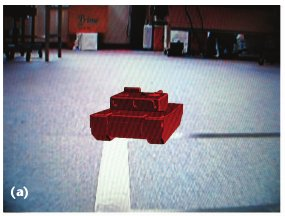
\includegraphics[width=200pt]{img/virtual_exocentric.jpg}  %robot pic
    \caption{A virtual exocentric vision example}
    \label{fig:virtualexocentric}
  \end{center}
\end{figure}

Key issues of such a system are:

\begin{itemize}
\item how to choose the \textit{best} image
\item how to determine the \textit{right} place to draw the robot
\end{itemize}

As for the first issue, the \textit{best} image is the one that allows 
the generation of the \textit{most comprehensible} external robot view.
\cite{sugimoto} provides a set of three effective metrics to 
determine which, of a set of previously recorded images, is the 
one to be chosen.
\\
Once the image is chosen, where to overlap the 3D robot representation 
is quite complex. It is not only a matter of \textit{where} draw the robot
on the image, but also of \textit{how} to set up lighting, robot dimensions,
perspective to make the end user not aware of the fact that what he is
seeing is not the actual environment.
\\
The issues introduced above will be deeply analyzed in the following 
of this document.



\section{Setting up a 3morduc simulator}
\label{sec:simulator}

In order to implement the exocentric vision \ref{sec:exo} we need a wide set of data provided by the robot.
This information consists of the camera images (the egocentric point of view) and of a simple textual file filled with 
the robot status. The latter let us know the robot position and its odometric data, because it would be impossible to draw 
the robot with Augmented Reality (AR) without this knowledge.
\newline The exocentric vision operates better with a large static space where the robot can move in. Since the real robot 
(named 3morduc) can not be easily teleguided in wide environment because of its size and the lack of a large room in Catania, 
where the robot is situated, a simulator has been used to reproduce the best set of data. The simulator can be thought of as 
a server, which receives requests and returns responses: the first are the commands sent by the user to move the robot, the
latter the egocentric images and the robot position data.
\newline Furthermore, with a simulator is extremely easy to change the environment where the robot is teleguided, so we can test
the exocentric vision with an infinite number of environments without physically moving the robot in different places. In this way
software development of exocentric vision can be faster, because it is simple and immediate to establish several test cases.
\newline The first simulator adopted was named 'Rosen'. Written in Erlang language, Rosen has been developed at the University
of Catania in order to simulate the behavior of robot with features completely different from 3morduc. The chief one was that
the robot had its own algorithm to set its movement, it was indeed not guided by a human operator.
\newline Rosen was used a couple of years ago for robot taking part in Euro-robot competition, but for our purpose was not fit
since it does not even provide a egocentric vision. The difficulties faced to edit Rosen made us to look for a more suitable
simulator.
\newline In 2006, at the Aalborg University, the Italian student Filippo Privitera wrote a simulator to teleguide the
3morduc robot \cite{privitera}. The simulator reproduces the robot (drawing its physical features) situated in a room with a
variable numbers of walls. Walls' position is specified by the user, by giving the simulator a black and white bitmap image
with the room plane to build the whole environment from.
\newline Besides, Privitera's simulator allows to enable the stereoscopic vision, with anaglyph or polarized method (both 
types are applied on the egocentric camera). These features make not too tricky to implement the exocentric vision control with 3d
effect, in order to improve the user's ability in moving the robot. Other information like the number of collisions or the robot
distance from the nearest obstacle are provided by simulator.
\newline This simulator was written in MFC (Microsoft Foundation Class) framework and has been used for testing user ability in
driving the robot, in comparison with the real robot server to quantify the differences between the two facilities. For more
information see \cite{privitera}.
\newline With a simulator specifically built for the 3morduc robot, it was not difficult to edit the source code to obtain what we 
needed. First of all, we needed to record data about egocentric vision and robot status, because they are the input value 
of the exocentric vision simulator. In order to achieve this, we edited the source code to allows the user to store data: by
pressing the 'P' key keyboard the actual information (e.g. the actual camera image and robot status) are recorded in
log files.
\newline Every session in Privitera's simulator has its own identifier (a integer number). When the 'P' key is pressed the
simulator write a new line in the text file named 'data< number of session >', creating the file if it does not exist. Each
line contains four float number values, with the following meaning:
\newline
\newline 1. x coordinate
\newline 2. y coordinate
\newline 3. theta value (in radiant s)
\newline 4. timestamp
\newline 
\newline The timestamp refers to the beginning of the simulation.
\newline Beside the text file there are several bitmap files, each for every line written in 'data <number of session>'. These 
files are named 'screenshot<number of session> <timestamp>', where the number of session indicates for every screenshot (e.g.
the egocentric vision) the proper text file, and the timestamp the line with the associated status of the robot.
\newline The software which implement the exocentric vision control will look for text and image files related to a specific 
session, in order to read the necessary input and draw the robot correctly. It must be able to choose the right image to use as 
background, among those previously read; to draw the robot over the background in the right position and orientation, depending 
on its route; to prevent or signal collisions to the user, and so on.
\newline Future development can reach a more interactive collaboration between simulator and exocentric vision control program. For
example, it would be better if the control program could interact (by a socket or another data stream) with the simulator, sending
the movement command and retrieving information about robot status. In this case log files would be substituted by a local or 
global connection, and the exocentric program would not read information from file (as it actually does) but from the network.
Furthermore, with log files the robot route is statically decided when they are created. With a network connection user
could teleguide the robot in real time, without caring if on the server side is present the simulator or the real robot 3morduc.

\subsection{Intro}
\frame
{
  \frametitle{Intro}
  
  \emph{\textit{R.E.A.R.} is a framework for the
    development of \textit{virtual exocentric vision systems}.}
  \pause
  
  \vskip15pt


  \begin{block} {\alert{\texttt{How it works}}}
    \begin{enumerate}

      \footnotesize

      \pause
      \item \texttt{take command input from user}
      \pause
      \item \texttt{send command to robot}
      \pause
      \item \texttt{retrieve robot position \& new egocentric image}
      \pause
      \item \texttt{add image to images' collection}
      \pause
      \item \texttt{choose the proper image to use as background}
      \pause
      \item \texttt{move the camera accordingly to the image chosen}
      \pause
      \item \texttt{move robot in its current position}
      
    \end{enumerate}
      
  \end{block}
      
}

\subsection{Independence from lower details}
\frame
{
  \frametitle{Independence from lower details}
  
  \emph{
    \textit{R.E.A.R.} exploits some object-oriented properties, such as \alert{polymorphism}
    and \alert{inheritance}, in order to work regardless of specific and low level details.
  }

  \vskip10pt
  \pause

  \begin{block} {\alert{\texttt{Lower details}}}
    \begin{itemize}

    \item \alert{\textit{how to draw the robot 3D model}} \\
      \pause

      \vskip5pt
      \only<3>{\footnotesize{user specifies a subclass of \alert{\texttt{Robot}} class: \\

          \begin{description} [\texttt{DrawRobot()}]

            \item [\texttt{DrawRobot()}]
              encapsulates how to draw the robot, through \textit{OpenGL} calls.

          \end{description}
        }}


      \pause

    \item \alert{\textit{how to choose the proper egocentric image}} \\
      \pause

      \vskip5pt
      \only<5>{\footnotesize{user specifies an implementation of \alert{\texttt{IImageSelector}} interface: \\

          \begin{description} [\texttt{ChoseImage()}]

            \item [\texttt{ChoseImage()}]
              encapsulates the exocentric image selection algorithm, given the current
              robot position and previous shot images' set.
          \end{description}
        }}
          
      \pause

    \item \alert{\textit{how to send and retrieve data to/from robot}} \\

      \pause
      \vskip5pt
      \only<7>{\footnotesize{user specifies an implementation of \alert{\texttt{IDataLogic}} interface: \\

          \begin{description} [\texttt{RetrieveData()}]
            \item [\texttt{SelectImage()}]
              delegates exocentric image selection to proper object; 
            \item [\texttt{RetrieveData()}]
              encapsulates how to read new status (i.e. position and egocentric
              image) from robot;
            \item [\texttt{Command()}]
              encapsulates how to send a movement command (forward, backward,
              left, right) to robot.
          \end{description}
        }}

      \pause

    \end{itemize}
    
  \end{block}
}


%%     \include{eurobot} % Eurobot Competition
%%     \include{bdi} % BDI
%%     \include{agentspeak} % AgentSpeak
%%     \include{masahiro} % Framework
%%     \include{casestudy} % Case Study
	

% Bibliography with BibTeX

\addcontentsline{toc}{section}{Bibliography}
\bibliography{biblio}
\bibliographystyle{style/IEEEtran}

\end{document}
